%
% Portuguese-BR vertion
% 
\documentclass{article}

\usepackage{ipprocess}
% Use longtable if you want big tables to split over multiple pages.
% \usepackage{longtable}
\usepackage[utf8]{inputenc} 
\usepackage[brazil]{babel} % Uncomment for portuguese

\sloppy

\graphicspath{{./pictures/}} % Pictures dir
\makeindex
\begin{document}

\DocumentTitle{Documento de Casos de Uso}
\Project{Core-MUSA}
\Organization{Universidade Estadual de Feira de Santana}
\Version{Build 3}

\capa
\newpage

%%%%%%%%%%%%%%%%%%%%%%%%%%%%%%%%%%%%%%%%%%%%%%%%%%
%% Revision History
%%%%%%%%%%%%%%%%%%%%%%%%%%%%%%%%%%%%%%%%%%%%%%%%%%
\section*{\center Histórico de Revisões}
  \vspace*{1cm}
  \begin{table}[ht]
    \centering
    \begin{tabular}[pos]{|m{2cm} | m{7.2cm} | m{3.8cm}|} 
      \hline
      \cellcolor[gray]{0.9}
      \textbf{Date} & \cellcolor[gray]{0.9}\textbf{Descrição} & \cellcolor[gray]{0.9}\textbf{Autor(s)}\\ \hline
      \hline
      \small 08/10/2014 & \small Concepção do documento & \small 
      \begin{itemize}
      	\item bezourokq;
      	\item wsbittencourt;
      	\item fmbboaventura;  
	  \end{itemize}      	
      \\ \hline
      \small 13/10/2014 & \small Build 2: Novo modelo de caso de uso & \small 
      \begin{itemize}
      	\item wsbittencourt;
      	\item jadsonfirmo;
      	\item fmbboaventura;  
	  \end{itemize}      	
      \\ \hline
      \small 16/10/2014 & \small Build 3: Novo modelo de caso de uso & \small 
      \begin{itemize}
      	\item wsbittencourt; 
	  \end{itemize}  
	  \\ \hline
	  \small 23/10/2014 & \small Revisão & \small 
      \begin{itemize}
      	\item jadsonfirmo; 
	  \end{itemize}  
	  \\ \hline
	  
	  \small 29/10/2014 & \small Inclusão Casos de Uso: JPC & \small 
	  \begin{itemize}
	  	\item di3goleite; 
	  \end{itemize}  
	  \\ \hline
	  
	  \small 29/10/2014 & \small Inclusão Casos de Uso: RET e NOP & \small 
      \begin{itemize}
      	\item mtcastro; 
	  \end{itemize}  
	  \\ \hline
	  
	  \small 30/10/2014 & \small Refatoração do documento & \small 
	  \begin{itemize}
	  	\item di3goleite; 
	  \end{itemize}  
	  \\ \hline
	  
    \end{tabular}
  \end{table}

\newpage

% TOC instantiation
\tableofcontents
\newpage

%%%%%%%%%%%%%%%%%%%%%%%%%%%%%%%%%%%%%%%%%%%%%%%%%%
%% Document main content
%%%%%%%%%%%%%%%%%%%%%%%%%%%%%%%%%%%%%%%%%%%%%%%%%%
\section{Introdução}
Este documento tem como objetivo a especificação dos casos de uso do projeto Core Musa (concepção de um processador simples de propósito geral). O documento detalha cada caso de uso indicando os atores, os eventos (ações) e as condições de cada caso, além dos diagramas de casos de uso.

  \subsection{Objetivo}
  
  \subsection{Visão Geral do Documento}
  \begin{itemize}
    \item Sessão 2: Lista todos os possíveis atores do sistema.
    \item Sessão 3: Relata a lista dos casos de uso do projeto.
    % \item Referências: provê uma lista completa de todos os artefatos referenciados nesse documento.
  \end{itemize}
  
  \subsection{Representação Simbólica}
  A Figura \ref{fig:uc_exemple} ilustra a simbologia utilizada para representar operações que devem ser realizadas pelo sistema. A Figura \ref{fig:actors} apresenta os modelos de ilustração utilizados para representar os Atores do sistema. Um ator, dentro do escopo desta descrição, pode ser identificado como um módulo \textit{top level}, ou como um elemento de entrada e saída (botões, sensores, \textit{displays}, etc).
  
  \FloatBarrier
  \begin{figure}[H]
    \centering
    
\includegraphics[width=0.25\textwidth]{uc_exemple.png}
    \caption{Exemplo de Caso de Uso.}
    \label{fig:uc_exemple}
  \end{figure}
  
  A simbologia usual para representação de um Ator é apresentada na Figura \ref{fig:actor_exemple}, no entanto, para representar módulos incorporados, utiliza-se as representações ilustradas nas Figuras \ref{fig:ipcore_exemple} e \ref{fig:ipcore_single_exemple}, definidas por convenção. Este elemento, em geral, está associado aos módulos do sistema, ou IP cores de terceiros incorporados ao mesmo. Esta simbologia foi divida, com o objetivo de representar instâncias únicas (Figura \ref{fig:ipcore_single_exemple}), ou múltiplas (Figura \ref{fig:ipcore_exemple}) de um determinado componente. 
  
  \FloatBarrier
  \begin{figure}[H]
    \centering
    \begin{subfigure}[b]{0.3\textwidth}
      \centering
      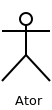
\includegraphics[width=0.25\textwidth]{actor_exemple.png}
      \caption{Ator do Sistema.}
      \label{fig:actor_exemple}
    \end{subfigure} 
    \begin{subfigure}[b]{0.3\textwidth}
      \centering
      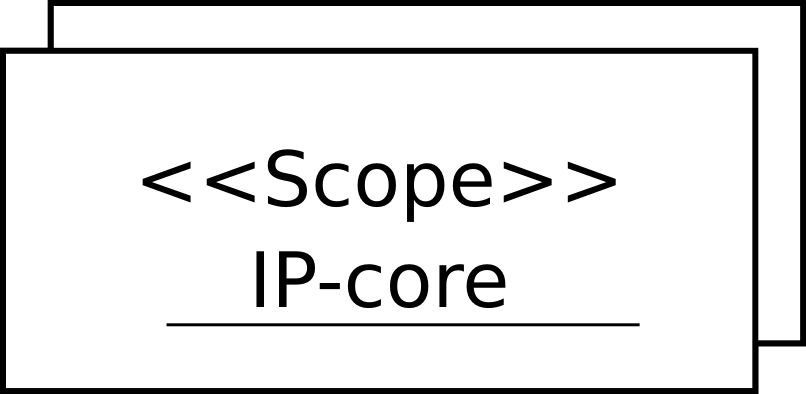
\includegraphics[width=0.6\textwidth]{ipcore_exemple.png}
      \caption{Instância múltipla de um IP.}
      \label{fig:ipcore_exemple}
    \end{subfigure}
    \begin{subfigure}[b]{0.3\textwidth}
      \centering
      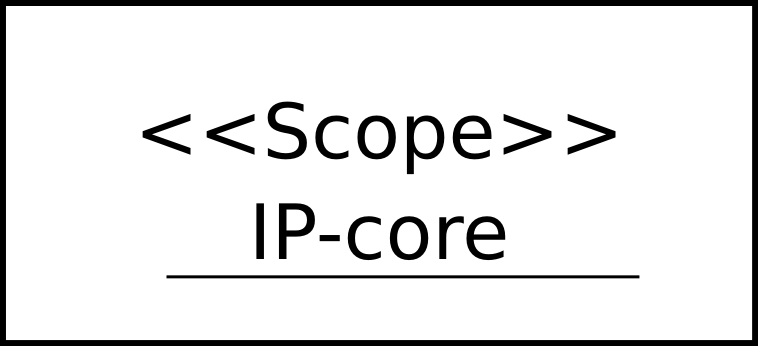
\includegraphics[width=0.6\textwidth]{ipcore_single_exemple.png}
      \caption{Instância de um IP.}
      \label{fig:ipcore_single_exemple}
    \end{subfigure}
    \caption{Simbologia utilizada na implementação dos Casos de Uso.}
    \label{fig:actors}
  \end{figure}
  
  O projetista responsável por interpretar os diagramas não deve confundir-se no momento de analisar as simbologias de atores. A representação alternativa, não implica que o módulo será instanciado no subsistema em questão, mas sim que os recursos providos por este \textit{core} são necessários para garantir o seu funcionamento.
  
  \subsection{Definições, Acrônimos e Abreviações}
  \FloatBarrier
    \begin{table}[H] 
      \begin{center}
        \begin{tabular}[pos]{|m{2cm} | m{8cm}|} 
          \hline 
          \cellcolor[gray]{0.9}\textbf{Termo} & \cellcolor[gray]{0.9}\textbf{Descrição} \\ \hline
          UC & Caso de Uso  \\ \hline
          ALU & Unidade Lógica e Aritmética \\ \hline
          SB & Sub-fluxo \\ \hline
          FS & Fluxo Secundário \\ \hline
          NFR & Requisito Não Funcional \\ \hline
          FR & Requisito Funcional \\ \hline
          BT & Botão Direcional \\ \hline
          PC & \textit{Program Counter} \\
          \hline
        \end{tabular}
      \end{center}
    \label{tab:definicoes}
    \end{table}

  \section{Atores do Sistema}
  
\begin{figure}[htb]
\centering
\begin{minipage}[c]{0.19\linewidth}
\centering
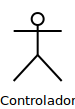
\includegraphics[scale=0.50]{./pictures/use/atores/controlador.png}
\end{minipage}
\begin{minipage}[c]{0.19\linewidth}
\centering
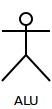
\includegraphics[scale=0.50]{./pictures/use/atores/alu.png}
\end{minipage}
\end{figure}

\textbf{Controlador} – Unidade que controla a execução das operações.

\textbf{ALU} – Unidade L\'{o}gica e Aritm\'{e}tica.
  
  \section{Casos de Usos}
  Esta sessão apresenta o conjunto de UC realizados para a implementação do projeto \textit{Core }MUSA (Núcleo de processamento de instruções do processador de propósito geral MUSA). As sessões a seguir foram divididas e nomeada utilizando a nomenclatura abreviada [UC (NÚMERO DO UC)] seguido de uma breve descrição em forma de título.

  \usecase{Execução de instruções}
  O controlador é responsável por decodificar instrução, solicitar operações na ALU e garantir o armazenamento dos resultados das operações no banco registradores.
  
  \actors
    \begin{description}
     \item \textbf{Controlador} – Unidade que controla a execução das operações.
     \item \textbf{ALU} – Unidade L\'{o}gica e Aritm\'{e}tica.
    \end{description}
    
  \preconditions 
    \begin{itemize}
     \item Atender aos requisitos funcionais [FR01 e FR02];
     \item Leitura do PC;
     \item Realizar operações lógicas e aritméticas na ALU;
    \end{itemize}

  \postconditions
    \begin{itemize}
     \item Os resultados devem ser expressos nos registradores.
    \end{itemize}

  \ucdiagram{./pictures/use/case/new.png}
  
  % descricao do fluxo principal de eventos
  \begin{mainflow}
    \item Acesso ao PC;
    \item Leitura da instrução apontada por PC;
    \item Acesso aos respectivos registradores;
    \item Executa operações;
    \item Atualiza registradores;
    \item Atualiza valor do PC;
  \end{mainflow}

  \usecase{BRFL}
  O Processador tem a capacidade de fazer desvios condicionais atrav\'{e}s da utilização das flags do sistema.
  \actors
    \begin{description}
     \item \textbf{Controlador} – Unidade que controla a execução das operações.
     \item \textbf{ALU} – Unidade L\'{o}gica e Aritm\'{e}tica.
    \end{description}
    
  \preconditions 
    \begin{itemize}
     \item Atender ao requisito funcional [FR14];
     \item Leitura do PC;
     \item Realizar operações lógicas na ALU;
    \end{itemize}

  \postconditions
    \begin{itemize}
     \item Alteração do PC caso verdadeira.
    \end{itemize}
  
  \ucdiagram{./pictures/use/case/brfl.png}
  
  % descricao do fluxo principal de eventos
  \begin{mainflow}
    \item Acesso ao PC;
    \item Leitura da instrução apontada pelo PC;
    \item Identificação e leitura da \textit{Flag} ativa;
    \item Executa a operação lógica;
    \item Atualiza o valor do PC;
  \end{mainflow}
  
  \usecase{Instrução LW}
  O processador é capaz de carregar dados da memória pro banco de registradores.
  \actors
    \begin{description}
     \item \textbf{Controlador} – Unidade que controla a execução das operações.
     \item \textbf{ALU} – Unidade L\'{o}gica e Aritm\'{e}tica.
    \end{description}
    
  \preconditions 
    \begin{itemize}
     \item Leitura da Memória de instrução;
     \item A instrução necessita ter o \textit{opcode} específico para a instrução LW;
    \end{itemize}

  \postconditions
    \begin{itemize}
     \item O dado deverá ser salvo no registrador de escrita (RD) do banco de registradores;
    \end{itemize}
  
  \ucdiagram{./pictures/use/case/LW_use_case.png}
  
  % descricao do fluxo principal de eventos
  \begin{mainflow}
    \item Decodificação da instrução lida na Memória de Programa;
    \item Acesso aos respectivos registradores;
	\item Leitura do endereço base, a partir do registrador RT;
	\item Extensão do valor de 16 bits lido na instrução para 32 bits;
	\item Operação de soma com os dados de 32 bits, dado lido no registrador, com o valor de 16 bits estendido para 32 bits;
	\item Resultado da operação será lido pela memória de dados, que servirá como endereço de memória para ler o dado;
	\item O dado será enviado para o banco de registradores, e será escrito no registrador de escrita RD;

  \end{mainflow}
  
  \usecase{Instrução SW}
  O processador é capaz de escrever dados na memória.
  \actors
    \begin{description}
     \item \textbf{Controlador} – Unidade que controla a execução das operações.
     \item \textbf{ALU} – Unidade L\'{o}gica e Aritm\'{e}tica.
    \end{description}
    
  \preconditions 
    \begin{itemize}
     \item Leitura da Memória de instrução;
     \item A instrução necessita ter o \textit{opcode} específico para a instrução SW;
    \end{itemize}

  \postconditions
    \begin{itemize}
     \item O dado deverá ser escrito na memória de dados.
    \end{itemize}
  
  \ucdiagram{./pictures/use/case/SW_use_case.png}
  
  % descricao do fluxo principal de eventos
  \begin{mainflow}
    \item Decodificação da instrução lida na Memória de Programa;
	\item Acesso aos respectivos registradores;
	\item Leitura do endereço base, a partir do registrador RT;
	\item Leitura do dado a ser escrito no registrador RS;
	\item Extensão do valor de 16 bits, lido na instrução, para 32 bits;
	\item Operação de soma com os dados de 32 bits com os seguintes valores: endereço lido do registrador RT e valor de 32 bits estendido;
	\item Resultado da operação será lido pela Memória de Dados, que servirá como endereço de memória para escrever o dado.
	\item O dado será escrito na Memória de Dados.
  \end{mainflow}
  
	\usecase{CALL}
	O Processador deve ser capaz de desviar um programa em execução para uma subrotina.
	
	\actors
	\begin{description}
		\item \textbf{Controlador} – Unidade que controla a execução das operações.
	\end{description}
	
	\preconditions 
	\begin{itemize}
		\item Atender ao requisito funcional [FR15];
		\item Leitura do PC;
		\item Ter espaço disponível na pilha de memória;
	\end{itemize}
	
	\postconditions
	\begin{itemize}
		\item Alteração do PC.
	\end{itemize}

	\newpage
	
	\ucdiagram{./pictures/use/case/call.png}
	
	% descricao do fluxo principal de eventos
	\begin{mainflow}
		\item Acesso ao PC;
		\item Leitura da instrução apontada por PC;
		\item Salvar o endereço atual do PC na pilha de memória;
		\item Modifica o valor do PC para o endereço recebido pela instrução;
	\end{mainflow}
  
  \usecase{JR}
  O Processador deve ser capaz de desviar um programa em execução para um endereço de destino.
  \actors
    \begin{description}
     \item \textbf{Controlador} – Unidade que controla a execução das operações.
    \end{description}
    
  \preconditions 
    \begin{itemize}
     \item Atender ao requisito funcional [FR12];
     \item Leitura do PC;
    \end{itemize}

  \postconditions
    \begin{itemize}
     \item Alteração do PC.
    \end{itemize}
  
  \ucdiagram{./pictures/use/case/jr.png}
  
  % descricao do fluxo principal de eventos
  \begin{mainflow}
    \item Acesso ao PC;
    \item Leitura da instrução apontada pelo PC;
    \item Modifica o valor do PC pro endereço recebido na instrução;
  \end{mainflow}
  
  \usecase{JPC}
  O processador deve ser capaz de desviar um programa em execução para um endereço relativo ao PC.
  \actors
  \begin{description}
  	\item \textbf{Controlador} – Unidade que controla a execução das operações.
  \end{description}
  
  \preconditions 
  \begin{itemize}
  	\item Leitura do PC;
  \end{itemize}
  
  \postconditions
  \begin{itemize}
  	\item Alteração do PC.
  \end{itemize}
  
  \ucdiagram{./pictures/use/case/jpc.png}
  
  % descricao do fluxo principal de eventos
  \begin{mainflow}
  	\item Acessa o valor de PC;
  	\item Faz a leitura da instrução apontada pelo PC;
  	\item Modifica o valor do PC pro endereço recebido na instrução;
  \end{mainflow}
  
  \usecase{Instruções  L\'{o}gicas e Aritm\'{e}ticas.}
  O controlador é responsável por decodificar instrução, solicitar operações na ALU e garantir o armazenamento dos resultados das operações no banco registradores.
  
  \actors
    \begin{description}
     \item \textbf{Controlador} – Unidade que controla a execução das operações.
     \item \textbf{ALU} – Unidade L\'{o}gica e Aritm\'{e}tica.
    \end{description}
    
  \preconditions 
    \begin{itemize}
     \item Atender aos requisitos funcionais [FR03 a FR10];
     \item Leitura do PC;
     \item Realizar operações lógicas e aritméticas na ALU;
    \end{itemize}

  \postconditions
    \begin{itemize}
     \item Os resultados devem ser expressos nos registradores.
    \end{itemize}
  
  \ucdiagram{./pictures/use/case/UC-ULA.jpeg}
  
  % descricao do fluxo principal de eventos
  \begin{mainflow}
    \item Acesso ao PC;
    \item Leitura da instrução apontada por PC;
    \item Acesso aos respectivos registradores;
    \item Controlador direciona os dados dos registradores para a entrada da ULA;
    \item Controlador envia o \textit{function} para ativar a operação desejada na ULA;
    \item A ULA realiza as operações;
    \item \textit{Flags} são disparadas, caso seja necessário;
    \item Envia o resultado pro registrador de destino;
  \end{mainflow}
  
  \usecase{RET}
  O processador deve ser capaz de retornar do último desvio tomado pelo programa.
  \actors
  \begin{description}
  	\item \textbf{Controlador} – Unidade que controla a execução das operações.
  \end{description}
  
  \preconditions 
  \begin{itemize}
  	\item Atender ao requisito funcional [FR15];
  	\item Leitura do PC;
  \end{itemize}
  
  \postconditions
  \begin{itemize}
  	\item Alteração do PC.
  \end{itemize}
  
  \ucdiagram{./pictures/use/case/ret.png}
  
  % descricao do fluxo principal de eventos
  \begin{mainflow}
  	\item Acesso ao PC;
  	\item Leitura da instrução apontada pelo PC;
  	\item Leitura do endereço do topo da pilha;
  	\item Remoção do endereço do topo da pilha;
  	\item Incrementa o endereço removido do topo da pilha;
  	\item Modifica o valor do PC pro valor incrementado;
  \end{mainflow}
  
   \usecase{NOP}
  O processador deve ser capaz de realizar nenhuma operação durante cinco ciclos de \textit{clock}.
  \actors
  \begin{description}
  	\item \textbf{Controlador} – Unidade que controla a execução das operações.
  \end{description}
  
  \preconditions 
  \begin{itemize}
  	\item Atender ao requisito funcional [FR15];
  	\item Leitura do PC;
  \end{itemize}
  
  \postconditions
  \begin{itemize}
  	\item Alteração do PC.
  \end{itemize}
  
  \ucdiagram{./pictures/use/case/nop.png}
  
  % descricao do fluxo principal de eventos
  \begin{mainflow}
  	\item Acesso ao PC;
  	\item Leitura da instrução apontada pelo PC;
  	\item Modifica o valor do PC pro endereço da próxima instrução.
  \end{mainflow} 

% Optional bibliography section
% To use bibliograpy, first provide the ipprocess.bib file on the root folder.
% \bibliographystyle{ieeetr}
% \bibliography{ipprocess}

\end{document}
